\documentclass{beamer}
\usepackage{hyperref}
\usepackage[T1]{fontenc}
\usepackage{tikz}
\usepackage[utf8]{inputenc}  % 如果你是 pdflatex
\usepackage{emoji}
\usepackage{animate} %模拟动图
\newcommand\Background{%
\begin{tikzpicture}[remember picture,overlay]
\node[inner sep=0pt,outer sep=0pt,opacity=0.5]
  at (current page.center){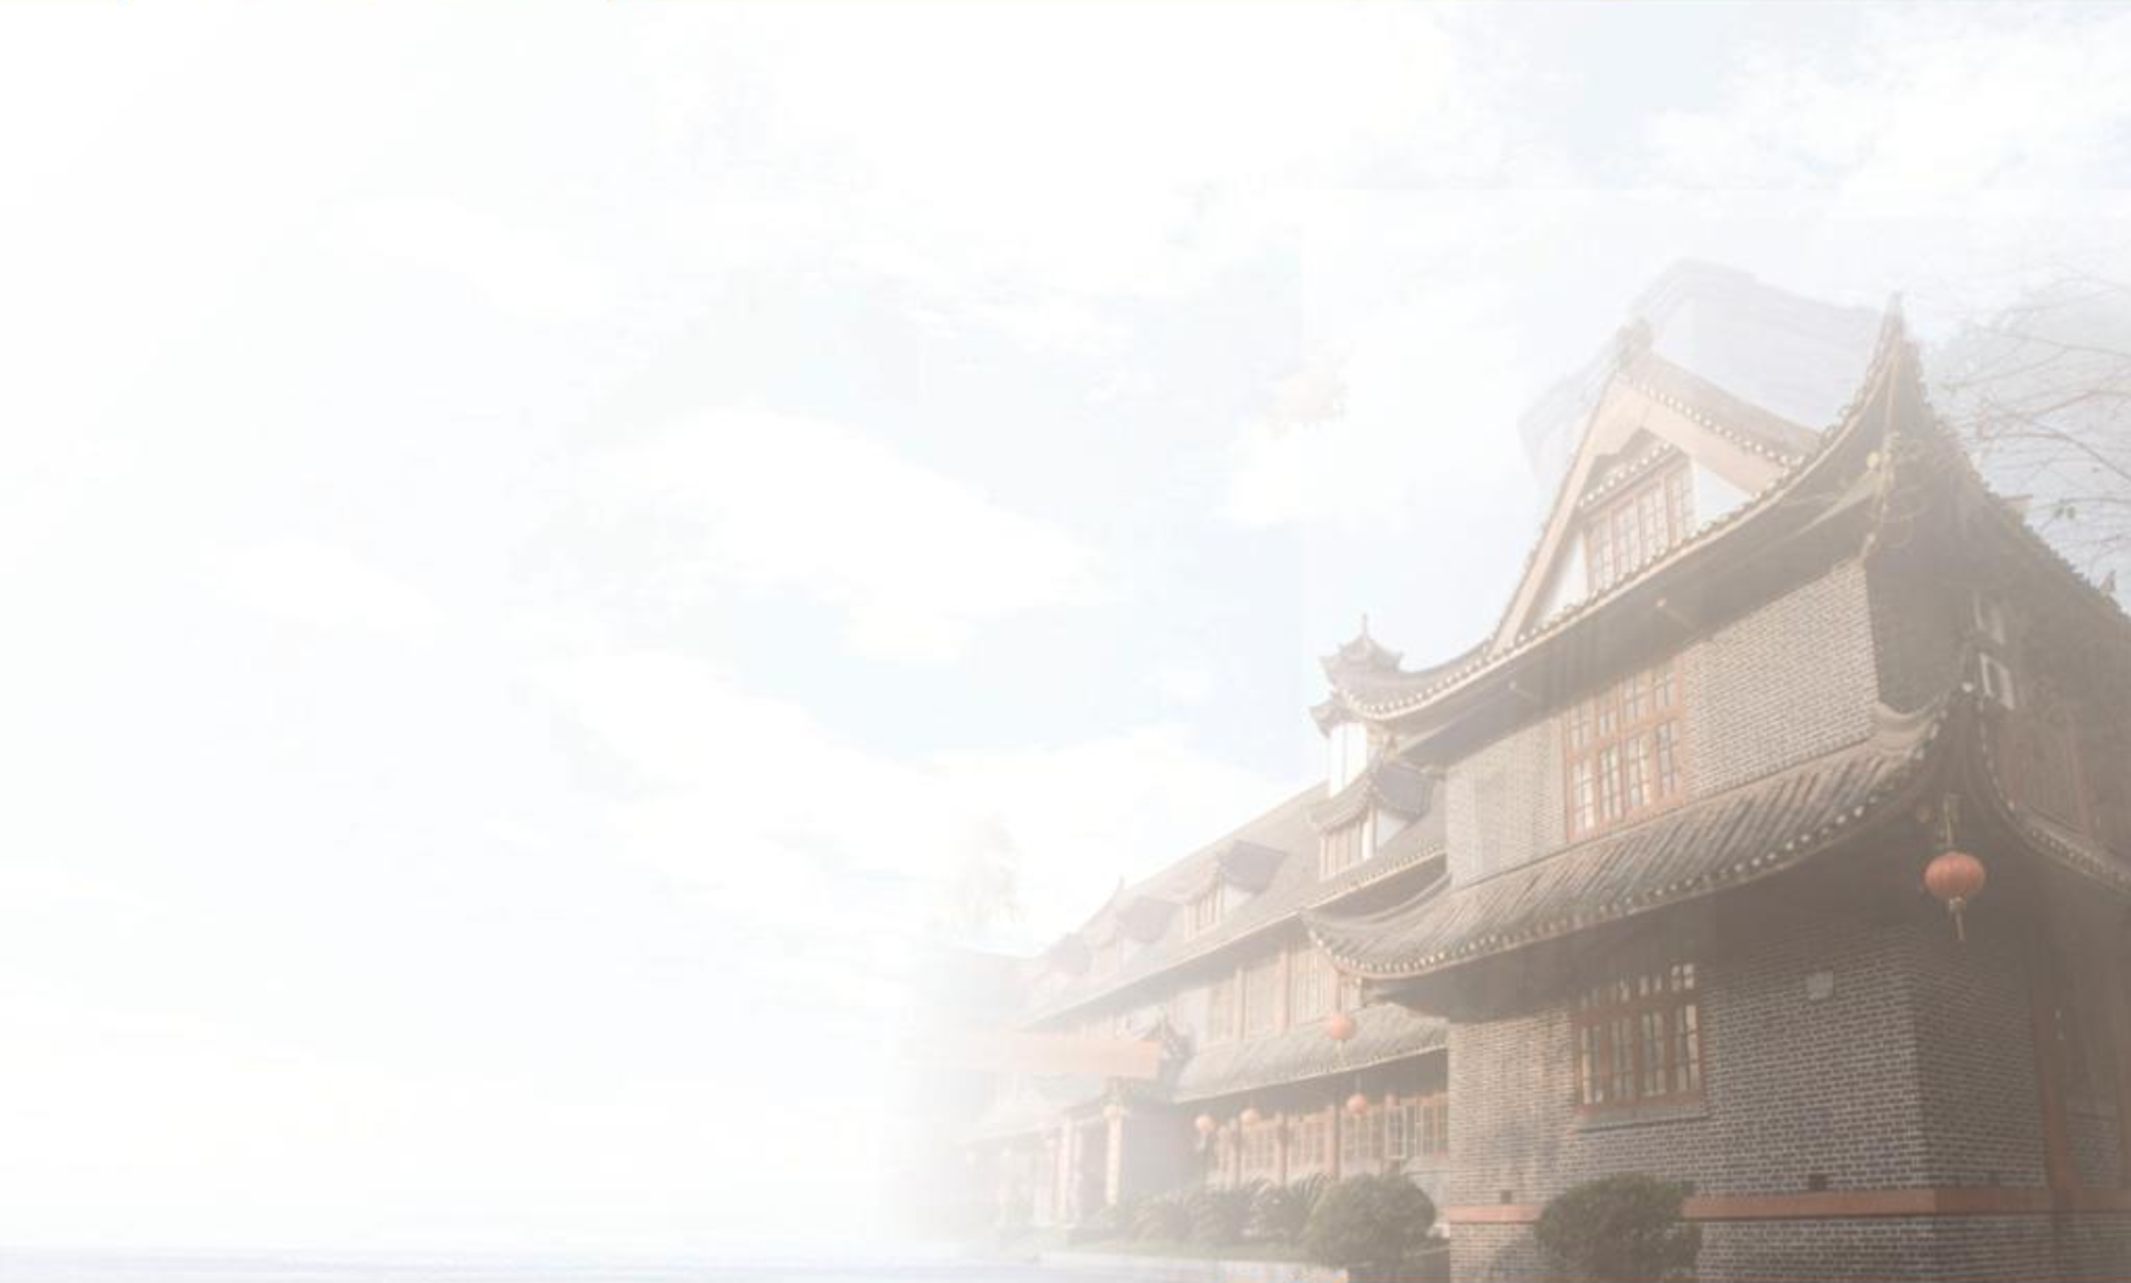
\includegraphics[width=1\paperwidth,height=1\paperheight]{fig/background.pdf}};
\end{tikzpicture}%
}
% other packages
\usepackage{latexsym,amsmath,xcolor,multicol,booktabs,calligra}
\usepackage{graphicx,pstricks,listings,stackengine}
\usepackage{cqu} % Assuming cqu.sty provides CQU specific commands/styles if needed elsewhere

% packages and settings for bibtex

\usefonttheme{serif}
\setbeamerfont{footnote}{size=\tiny}   % footnote for bibtex

\setbeamertemplate{bibliography item}[text]   % reference list for bibtex
\defbibheading{reference}{\section*{Reference}}   % heading for bibtex

\author[Haotian Yang]{Haotian Yang\\{\small younght@qq.com}}
\title{Intro to Optimal Control}
\subtitle{A (Biased) Brief Introduction} % <-- Updated Subtitle
\institute{College of Automation\\
  Chongqing University}
\date[2025] % (optional)
{Created on April 16, 2025} % <-- Updated Date

% defs
\def\cmd#1{\texttt{\color{red}\footnotesize $\backslash$#1}}
\def\env#1{\texttt{\color{blue}\footnotesize #1}}
\definecolor{cqublue}{RGB}{2,82,159} % Standard Color-CQU Blue
\definecolor{deepred}{rgb}{0.6,0,0}
\definecolor{deepgreen}{rgb}{0,0.5,0}
\definecolor{halfgray}{gray}{0.55}

\lstset{
    basicstyle=\ttfamily\small,
    keywordstyle=\bfseries\color{cqublue},
    emphstyle=\ttfamily\color{deepred},    % Custom highlighting style
    stringstyle=\color{deepgreen},
    numbers=left,
    numberstyle=\small\color{halfgray},
    rulesepcolor=\color{red!20!green!20!blue!20},
    frame=shadowbox,
}
\AtBeginSection[]{

  \begin{frame}
  \centering
  \begin{beamercolorbox}[sep=12pt,center]{part title}
  \usebeamerfont{section title}\insertsection\par
  \end{beamercolorbox}
  \end{frame}

}

\begin{document}

\begin{frame}
\Background
    \titlepage
    \begin{figure}[htpb]
        \begin{center}
            
\includegraphics[width=0.15\linewidth]{fig/Chongqing_University_Logo.pdf}
        \end{center}
    \end{figure}
\end{frame}

\begin{frame}{Outline} % Changed title from Table of Contents for clarity
        \begin{itemize}
            \item What is Optimal Control?
            \item Why Optimal Control?
            \item Key Concepts
            \begin{itemize}
                \item System dynamics and variables
                \item Cost functions and constraints
            \end{itemize}
            \item Common Methods
            \begin{itemize}
                \item Classical approaches
                \item Numerical techniques
            \end{itemize}
            \item Case Study: Newton's Method & KKT conditions
            \item Examples
            \begin{itemize}
                \item Aerospace applications
                \item Rocket landing and quadrotors
            \end{itemize}
            \item Summary
        \end{itemize}
\end{frame}

% --- Optimal Control Content Starts Here ---
\section{What is Optimal Control?}
\begin{frame}
\frametitle{What is Optimal Control?}
    \begin{itemize}
        \item Optimal control deals with finding a control strategy for a dynamic system over a period of time to achieve a specific objective optimally.
        \item What does "optimal" mean?
        \begin{itemize}
            \item Minimizing a cost function (e.g., time, fuel consumption, error).
            \item Maximizing a reward function (e.g., profit, distance covered, product yield).
        \end{itemize}
        \item It essentially answers the question: "How should I operate my system to achieve a goal in the \emph{best} possible way?"
        \item Requires balancing desired performance against system limitations and constraints.
    \end{itemize}
\end{frame}

\section{Why Optimal Control?}
\begin{frame}
\frametitle{Why Study Optimal Control? Applications}
    Optimal control principles are fundamental in many fields:
    \begin{itemize}
        \item \textbf{Aerospace Engineering:} Minimum-fuel or minimum-time spacecraft trajectories, missile guidance, aircraft flight control.
        \item \textbf{Robotics:} Path planning for robot arms or mobile robots (e.g., fastest path, least energy consumption).
        \item \textbf{Chemical Engineering:} Optimizing reactor conditions to maximize product yield or minimize operating costs.
        \item \textbf{Economics \& Finance:} Optimal resource allocation, investment strategies, inventory management.
        \item \textbf{Automotive:} Autonomous driving (path planning, speed control), hybrid vehicle energy management.
        \item \textbf{Power Systems:} Economic dispatch, load frequency control.
    \end{itemize}
\end{frame}

\section{Key Concepts}
\begin{frame}
\frametitle{Key Components of an Optimal Control Problem}
    \begin{itemize}
        \item \textbf{System Dynamics:} Mathematical model describing how the system's state evolves over time. Often represented by differential equations:
        $$ \dot{x}(t) = f(x(t), u(t), t) $$
        where $x$ is the state vector, $u$ is the control input vector

        \item \textbf{Control Inputs ($u$):} The variables we can manipulate or choose to influence the system's behavior.

        \item \textbf{State Variables ($x$):} Variables that characterize the condition or configuration of the system at any given time.

        \item \textbf{Cost Function (Objective Function, $J$):} A scalar value quantifying the performance. We aim to minimize (or maximize) this. A common form is:
        $$ J = \Phi(x(t_f), t_f) + \int_{t_0}^{t_f} L(x(t), u(t), t) dt $$
        ($\Phi$: terminal cost, $L$: running cost)

        \item \textbf{Constraints:} Limitations on states ($x$) or control inputs ($u$), e.g., actuator limits ($u_{min} \le u(t) \le u_{max}$), state boundaries, specific initial/final conditions.
    \end{itemize}
\end{frame}

\begin{frame}
\frametitle{Conceptual Example: Driving a Car}
    Imagine driving from Point A to Point B:
    \begin{itemize}
        \item \textbf{System Dynamics:} Physics of the car (position, velocity, acceleration based on engine/braking forces).
        \item \textbf{State Variables ($x$):} Position, velocity, fuel level.
        \item \textbf{Control Inputs ($u$):} Steering angle, accelerator position, brake pressure.
        \item \textbf{Possible Objectives (Cost Functions $J$):}
        \begin{itemize}
            \item Minimize travel time: $J = t_f - t_0$.
            \item Minimize fuel consumption: $J = \int_{t_0}^{t_f} \text{fuel\_rate}(u(t)) dt$.
            \item Minimize discomfort (e.g., jerky movements): $J = \int_{t_0}^{t_f} (\text{acceleration}^2 + \text{jerk}^2) dt$.
        \end{itemize}
        \item \textbf{Constraints:} Speed limits, road boundaries, maximum acceleration/braking, car cannot go in reverse (usually!).
    \end{itemize}
    Optimal control finds the sequence of steering/accelerator/brake actions ($u(t)$) that achieves the chosen objective best, given the car's dynamics and constraints.
\end{frame}

\section{Common Methods}
\begin{frame}
\frametitle{How are Optimal Control Problems Solved?}
    Finding the optimal control $u^*(t)$ often involves advanced mathematical techniques:
    \begin{itemize}
        \item \textbf{Calculus of Variations:} The historical foundation, dealing with minimizing functionals (functions of functions).

        \item \textbf{Pontryagin's Maximum Principle (PMP):}
        \begin{itemize}
            \item Provides \emph{necessary conditions} for optimality.
            \item Introduces costate variables and a Hamiltonian function.
            \item Often leads to solving a two-point boundary value problem (TPBVP), which can be challenging.
        \end{itemize}

        \item \textbf{Dynamic Programming (DP):}
        \begin{itemize}
            \item Based on Bellman's Principle of Optimality ("An optimal policy has the property that whatever the initial state and initial decision are, the remaining decisions must constitute an optimal policy with regard to the state resulting from the first decision.")
            \item Leads to the Hamilton-Jacobi-Bellman (HJB) equation (a partial differential equation) for continuous-time systems.
            \item Powerful, especially for discrete-time or stochastic problems, but suffers from the "Curse of Dimensionality" (computationally expensive for high-dimensional state spaces).
        \end{itemize}

        \item \textbf{Numerical Methods:}
        \begin{itemize}
            \item \textbf{Direct Methods:} Discretize the control and/or state variables and convert the optimal control problem into a large (non-linear) optimization problem. Solved using standard numerical optimization techniques (e.g., SQP).
            \item \textbf{Indirect Methods:} Solve the necessary conditions derived from PMP (the TPBVP) numerically (e.g., using shooting methods).
        \end{itemize}
    \end{itemize}
\end{frame}

\section{Case Study}
\begin{frame}{Newton's Methods}
\begin{figure}[htbp]  
    % 开始一个浮动图形环境,LaTeX 会根据 [htbp] 建议安排图的位置:
    % h: 尽量在当前位置 (here)
    % t: 页顶 (top)
    % b: 页底 (bottom)
    % p: 单独的浮动页 (page of floats)

    \centering
    % 使图片在页面中居中显示

    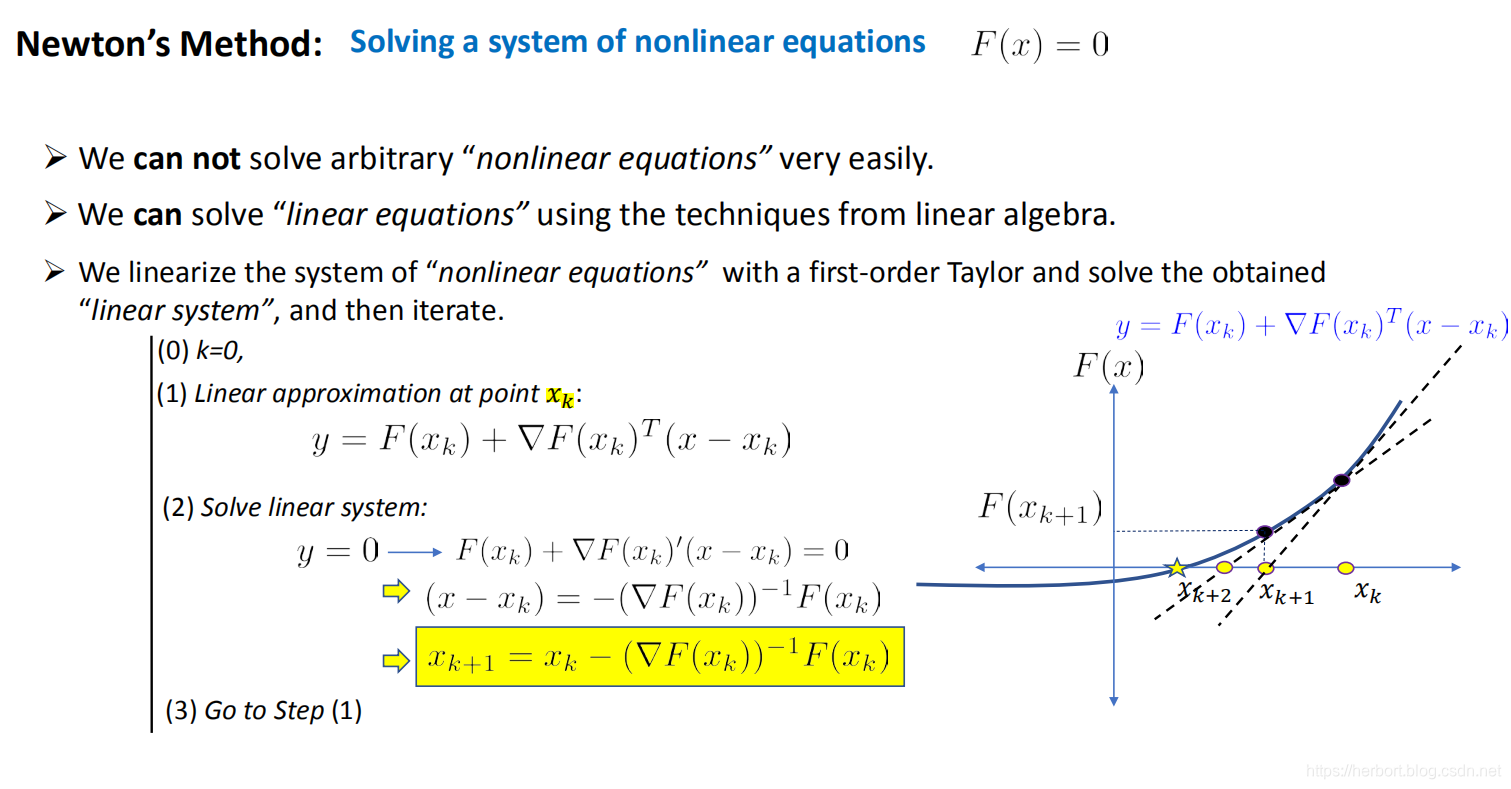
\includegraphics[width=1\textwidth]{fig/newton_method.png}
    % 插入图片,宽度为正文宽度的 80%
    % 图片路径是相对于主 tex 文件的,相当于 fig 文件夹中的 myfigure.png

    %\caption{}
    % 图像标题,会自动编号并出现在图下方,也会出现在图目录中(若有)

    % 设置该图的标签,可以用于交叉引用,如 \ref{fig:example}

\end{figure}
% 结束浮动图形环境
\end{frame}

\begin{frame}{KKT condition}
\[
\begin{aligned}
\min_{x_{1:N},\, u_{1:N-1}} \quad & \left[ \sum_{i=1}^{N-1} \ell(x_i, u_i) \right] + \ell_N(x_N) \\
\text{s.t.} \quad & x_1 = x_{\mathrm{IC}} \\
& x_{k+1} = f(x_k, u_k), \quad \text{for } k = 1,2,\ldots,N-1
\end{aligned}
\]    
\end{frame}

\begin{frame}{KKT condition}
\footnotesize
We are going to solve an equality-constrained optimization problem:
\[
\begin{aligned}
\min_x \quad & f(x) \\
\text{s.t.} \quad & c(x) = 0
\end{aligned}
\]
\vspace{0.5em}
The Lagrangian of the problem is defined as:
\[
\mathcal{L}(x,\lambda) = f(x) + \lambda^T c(x)
\]
The corresponding KKT conditions for optimality are:
\[
\begin{aligned}
\nabla_x \mathcal{L} &= \nabla_x f(x) + \left( \frac{\partial c}{\partial x} \right)^T \lambda = 0 \\
c(x) &= 0
\end{aligned}
\]
\vspace{0.5em}
This is essentially a \alert{root-finding problem}. We aim to solve for
\[
z = \begin{bmatrix} x \\ \lambda \end{bmatrix}
\]
such that the KKT conditions are satisfied.
\end{frame}

\begin{frame}{How to solve?}
\big
But, Do we really need to solve these complex math problems?

\end{frame}


\begin{frame}{How to solve?}
    \begin{columns}
        \column{0.3\textwidth}  % Left column
        \begin{center}
            
\includegraphics[width=0.8\textwidth]{fig/Julia.png}  % Julia logo
            \vspace{1em}
            \textbf{Julia}
            
            \begin{itemize}
                \item High-performance
                \item Easy to learn
                \item Powerful optimization
            \end{itemize}
        \end{center}
        
        \column{0.68\textwidth}  % Right column
        \begin{block}{Solving with JuMP}
            \footnotesize
            \begin{verbatim}
using JuMP, Ipopt

model = Model(Ipopt.Optimizer)

@variable(model, x[1:2])

@objective(model, Min, 
    (x[1] - 2)^2 + (x[2] - 3)^2)

@constraint(model, x[1] + x[2] == 1)

optimize!(model)
            \end{verbatim}
        \end{block}
    \end{columns}
\end{frame}
\section{Examples}
    
\begin{frame}{Aerospace}
    \footnotesize
    \[
    \begin{aligned}
    \min_{x_{0:N},\, u_{0:N-1}} \quad & \left[ \sum_{k=0}^{N-1} \|x_k - x_{ref}\|_Q^2 + \|u_k\|_R^2 \right] + \|x_N - x_{ref}\|_{Q_f}^2 \\
    \text{s.t.} \quad & x_0 = x_{\text{init}} \\
    & x_{k+1} = f(x_k, u_k), \quad k = 0,1,\ldots,N-1 \\
    & u_{min} \leq u_k \leq u_{max}, \quad k = 0,1,\ldots,N-1 \\
    & x_{min} \leq x_k \leq x_{max}, \quad k = 1,2,\ldots,N
    \end{aligned}
    \]
    
    \vspace{0.5em}
    
    where:
    \begin{itemize}
        \item $x_k$ is the state vector (e.g. position, velocity, attitude)
        \item $u_k$ is the control input (e.g. thrust, torque)
        \item $x_{ref}$ is the reference trajectory
        \item $Q$, $R$, $Q_f$ are weighting matrices
        \item $f(x_k, u_k)$ represents aircraft dynamics
        \item State and control constraints ensure safety and feasibility
    \end{itemize}
    
    \vspace{0.5em}
    \end{frame}

\begin{frame}{Rocket Landing}
\begin{columns}
    \column{0.48\textwidth}  % 左列,稍微小于一半宽度以留间隙
    \begin{figure}
        \centering
        \animategraphics[autoplay,loop,width=0.8\textwidth]{20}{fig/spaceship-}{0}{60}        
        \caption{Spaceship}
    \end{figure}
    
    \column{0.48\textwidth}  % 右列
    \begin{figure}
        \centering
        \animategraphics[autoplay,loop,width=0.8\textwidth]{20}{fig/rocket-}{0}{20}        
        \caption{Rocket Landing}
    \end{figure}
\end{columns}
\end{frame}

\begin{frame}{Quadrotors}
\[
\begin{aligned}
\min_{x_{1:N},\, u_{1:N-1}} \quad & \left[ \sum_{i=1}^{N-1} \ell(x_i, u_i) \right] + \ell_N(x_N) \\
\text{s.t.} \quad & x_1 = x_{\mathrm{IC}} \\
& x_{k+1} = f(x_k, u_k), \quad \text{for } k = 1,2,\ldots,N-1
\end{aligned}
\]

\vspace{0.5em}

where:
\begin{itemize}
    \item $x_{\mathrm{IC}}$ init;
    \item $x_{k+1} = f(x_k, u_k)$ dynamc;
    \item $\ell(x_i,u_i)$ cost;
    \item $\ell_N(x_N)$ finalcost。
    \item Safty Constraints
\end{itemize}

\vspace{0.5em}

\end{frame}

\begin{frame}{Quadrotors}
    \begin{figure}
        \centering
        \animategraphics[autoplay,loop,width=0.8\textwidth]{20}{fig/quadrotor-}{0}{20}        
        \caption{Quadrotors}
    \end{figure}
\end{frame}
% --- Optimal Control Content Ends Here ---

\section{Summary}

\begin{frame}
\frametitle{Summary}
    \begin{itemize}
        \item Optimal control is about finding the \emph{best} way to control a dynamic system according to a defined objective (cost function).
        \item It involves understanding the system's dynamics, defining what "best" means (the cost function), and respecting constraints.
        \item It has broad applications across science, engineering, and economics.
        \item Solutions often require sophisticated tools like PMP, Dynamic Programming, or numerical optimization techniques.
    \end{itemize}
\end{frame}

\begin{frame}{Reference}
    % Based on course materials from Carnegie Mellon University
    % 删除原来的注释和 \textit 部分
    
    \begin{thebibliography}{9}
        \bibitem{cmu-course} Zachary Manchester, ``16-745: Optimal Control,'' Carnegie Mellon University, 2023. Teaching Assistant: Kevin Tracy.
        
        \bibitem{kirk2004optimal} Donald E. Kirk, ``Optimal Control Theory: An Introduction,'' Dover Publications, 2004.
        
        \bibitem{manchester2018dirtrel} Zachary Manchester, Scott Kuindersma, ``DIRTREL: Robust Trajectory Optimization with Ellipsoidal Disturbances and LQR Feedback,'' Robotics: Science and Systems, 2018.
        
        \bibitem{nocedal2006numerical} Jorge Nocedal, Stephen J. Wright, ``Numerical Optimization,'' Springer Series in Operations Research, Second Edition, 2006.
    \end{thebibliography}
\end{frame}

\begin{frame}
\Background
    \begin{center}
        {\Huge Q\&A}\\
        \textit{Thank you!}\\
        \textit{Your feedback will be highly appreciated!}
    \end{center}
\end{frame}

\end{document}